\documentclass[12pt, twoside]{book}\usepackage[]{graphicx}\usepackage[]{color}
%% maxwidth is the original width if it is less than linewidth
%% otherwise use linewidth (to make sure the graphics do not exceed the margin)
\makeatletter
\def\maxwidth{ %
  \ifdim\Gin@nat@width>\linewidth
    \linewidth
  \else
    \Gin@nat@width
  \fi
}
\makeatother

\definecolor{fgcolor}{rgb}{0.345, 0.345, 0.345}
\newcommand{\hlnum}[1]{\textcolor[rgb]{0.686,0.059,0.569}{#1}}%
\newcommand{\hlstr}[1]{\textcolor[rgb]{0.192,0.494,0.8}{#1}}%
\newcommand{\hlcom}[1]{\textcolor[rgb]{0.678,0.584,0.686}{\textit{#1}}}%
\newcommand{\hlopt}[1]{\textcolor[rgb]{0,0,0}{#1}}%
\newcommand{\hlstd}[1]{\textcolor[rgb]{0.345,0.345,0.345}{#1}}%
\newcommand{\hlkwa}[1]{\textcolor[rgb]{0.161,0.373,0.58}{\textbf{#1}}}%
\newcommand{\hlkwb}[1]{\textcolor[rgb]{0.69,0.353,0.396}{#1}}%
\newcommand{\hlkwc}[1]{\textcolor[rgb]{0.333,0.667,0.333}{#1}}%
\newcommand{\hlkwd}[1]{\textcolor[rgb]{0.737,0.353,0.396}{\textbf{#1}}}%
\let\hlipl\hlkwb

\usepackage{framed}
\makeatletter
\newenvironment{kframe}{%
 \def\at@end@of@kframe{}%
 \ifinner\ifhmode%
  \def\at@end@of@kframe{\end{minipage}}%
  \begin{minipage}{\columnwidth}%
 \fi\fi%
 \def\FrameCommand##1{\hskip\@totalleftmargin \hskip-\fboxsep
 \colorbox{shadecolor}{##1}\hskip-\fboxsep
     % There is no \\@totalrightmargin, so:
     \hskip-\linewidth \hskip-\@totalleftmargin \hskip\columnwidth}%
 \MakeFramed {\advance\hsize-\width
   \@totalleftmargin\z@ \linewidth\hsize
   \@setminipage}}%
 {\par\unskip\endMakeFramed%
 \at@end@of@kframe}
\makeatother

\definecolor{shadecolor}{rgb}{.97, .97, .97}
\definecolor{messagecolor}{rgb}{0, 0, 0}
\definecolor{warningcolor}{rgb}{1, 0, 1}
\definecolor{errorcolor}{rgb}{1, 0, 0}
\newenvironment{knitrout}{}{} % an empty environment to be redefined in TeX

\usepackage{alltt}\usepackage[]{graphicx}\usepackage[]{color}

\usepackage{alltt}\usepackage[]{graphicx}\usepackage[]{color}
\usepackage[utf8]{inputenc}
\usepackage[spanish]{babel}
\usepackage{fancyhdr}
\usepackage{lastpage}
\usepackage{lscape} %Para seleccionar páginas horizontales 
\usepackage[cc]{titlepic} 
\usepackage[hidelinks]{hyperref}  %Para links ocultos
\usepackage{url} %Para direcciones web
\usepackage[makeroom]{cancel}
\pagestyle{fancy}
\usepackage{multicol} % muchas columnas
\usepackage{booktabs} % midrule, bottomrule
\usepackage{titlesec} % cambiar secuencias de TOC 
\let\bold\boldsymbol
\let\bf\mathbf


\fancyhf{}
 \setcounter{page}{1}
%\rfoot{Página \thepage \hspace{1pt} de \pageref{LastPage}}
\setcounter{section}{0}

\usepackage[caption=false]{subfig}
\usepackage{blindtext}  %Texo sin sentido
\usepackage{amsmath} \newenvironment{smatrix}{\left(\begin{smallmatrix}}{\end{smallmatrix}\right)} %SMALL
\usepackage{amsthm}
\usepackage{amsfonts}
\DeclareMathOperator{\sgn}{sgn} %Para formalizar la función signo 
\usepackage{enumerate}
\usepackage{dsfont} %Para usar una indicadora
\numberwithin{equation}{section}
\usepackage{xcolor}
\usepackage[backend=bibtex]{biblatex}
\bibliography{biblio.bib}
\usepackage{booktabs,caption}
\usepackage[flushleft]{threeparttable}

\usepackage{mdframed} %Para usar recuadros

    \usepackage{framed}

    \colorlet{shadecolor}{blue!15}

    \newtheorem{theorem}{Observación}
    \newenvironment{theo}
      {\begin{shaded}\begin{theorem}}
      {\end{theorem}\end{shaded}}
      \numberwithin{theorem}{section}

\colorlet{shadecolor}{red!15}

    \newtheorem{teorema}{Proposición}
    \newenvironment{teo}
      {\begin{shaded}\begin{teorema}}
      {\end{teorema}\end{shaded}}
      \numberwithin{teorema}{section}

\colorlet{shadecolor}{gray!15}
    \newtheorem{defi}{Definición}
    \newenvironment{defin}
      {\begin{shaded}\begin{defi}}
      {\end{defi}\end{shaded}}
      \numberwithin{defi}{section}
%\newtheorem{rexample}{Código R}[subsection]
\newtheorem{prop}{Proposición}
%\newtheorem{defi}{Definición}
\numberwithin{prop}{section}
\numberwithin{defi}{section}
\theoremstyle{plain}
\setlength{\textfloatsep}{10pt}
\usepackage{multicol}
\usepackage{float}

\usepackage[affil-it]{authblk}
\usepackage{setspace}
\usepackage{listings}

\usepackage{geometry}
\geometry{a4paper, left=3cm, right=3cm, top=3cm, bottom=3cm}
\newcommand*\rfrac[2]{{}^{#1}\!/_{#2}}
\title{Análisis de datos: Transmisión de precios}
\author{H\'ector Garrido Henr\'iquez\thanks{Ingeniero Comercial. Contacto: \texttt{hectorgarridohenriquez@gmail.com}} \\ 
Profesor: Sergio Contreras Espinoza}

\affil{Mag\'ister en Matem\'atica Menci\'on Estad\'istica \\ Universidad del B\'io-B\'io}
\IfFileExists{upquote.sty}{\usepackage{upquote}}{}

\allowdisplaybreaks
\IfFileExists{upquote.sty}{\usepackage{upquote}}{}
\IfFileExists{upquote.sty}{\usepackage{upquote}}{}
\IfFileExists{upquote.sty}{\usepackage{upquote}}{}
\begin{document}
%\SweaveOpts{concordance=TRUE}
\begin{titlepage}
\begin{center}

\includegraphics[scale=0.07]{./figure/logo.png}\\
\textsc{\Large Universidad del Bío-Bío \\[0.5cm] Facultad de Ciencias}\\[1cm] % University name
\textsc{\Large}\\[0.3cm] % Thesis type

\noindent\makebox[\linewidth]{\rule{\textwidth}{1pt}} 
{\huge Transmisi\'on Asim\'etrica de Precios en el sector de la palta en Chile:\\[0.3cm] Evidencia desde un modelo TVECM}\\[0.4cm] % Thesis title
\noindent\makebox[\linewidth]{\rule{\textwidth}{1pt}} 

\textsc{\Large}\\[0.5cm] % Thesis type

\begin{minipage}{0.45\textwidth}
\begin{flushleft} \large
\emph{Autor:}\\
Héctor Garrido Henríquez % Author name - remove the \href bracket to remove the link
\end{flushleft}
\end{minipage}
\begin{minipage}{0.45\textwidth}
\begin{flushleft} \large
\emph{Profesor(es) Guía(s):} \\
Dr. Sergio Contreras Espinoza \\ Dra. Monia Ben Kaabia 
\end{flushleft}
\end{minipage}\\[2cm]
 
\large \textit{Tesis para optar al grado de Magíster en Matemática con mención en Estadística}\\[0.3cm] % University requirement text
\textit{}\\[0.4cm]
\ Departamento de Estadística \\
[0.4cm]\ Departamento de Matemática
\\[1cm] % Research group name and department name
 
{\large \today}\\[2cm] % Date
%\includegraphics{Logo} % University/department logo - uncomment to place it
 
%\vfill
\end{center}

\end{titlepage}
\newpage



\tableofcontents

\listoffigures
\listoftables
\onehalfspacing
\chapter*{Agradecimientos}
\chapter*{Abstract}
\chapter{Introducción}
\section{introducción}
\section{justificación del trabajo}



\chapter{Análisis univariante de las series de precios}
\section{Fuentes de información}

\subsection{Imputación de valores perdidos}









\begin{knitrout}
\definecolor{shadecolor}{rgb}{0.969, 0.969, 0.969}\color{fgcolor}\begin{figure}[H]

{\centering 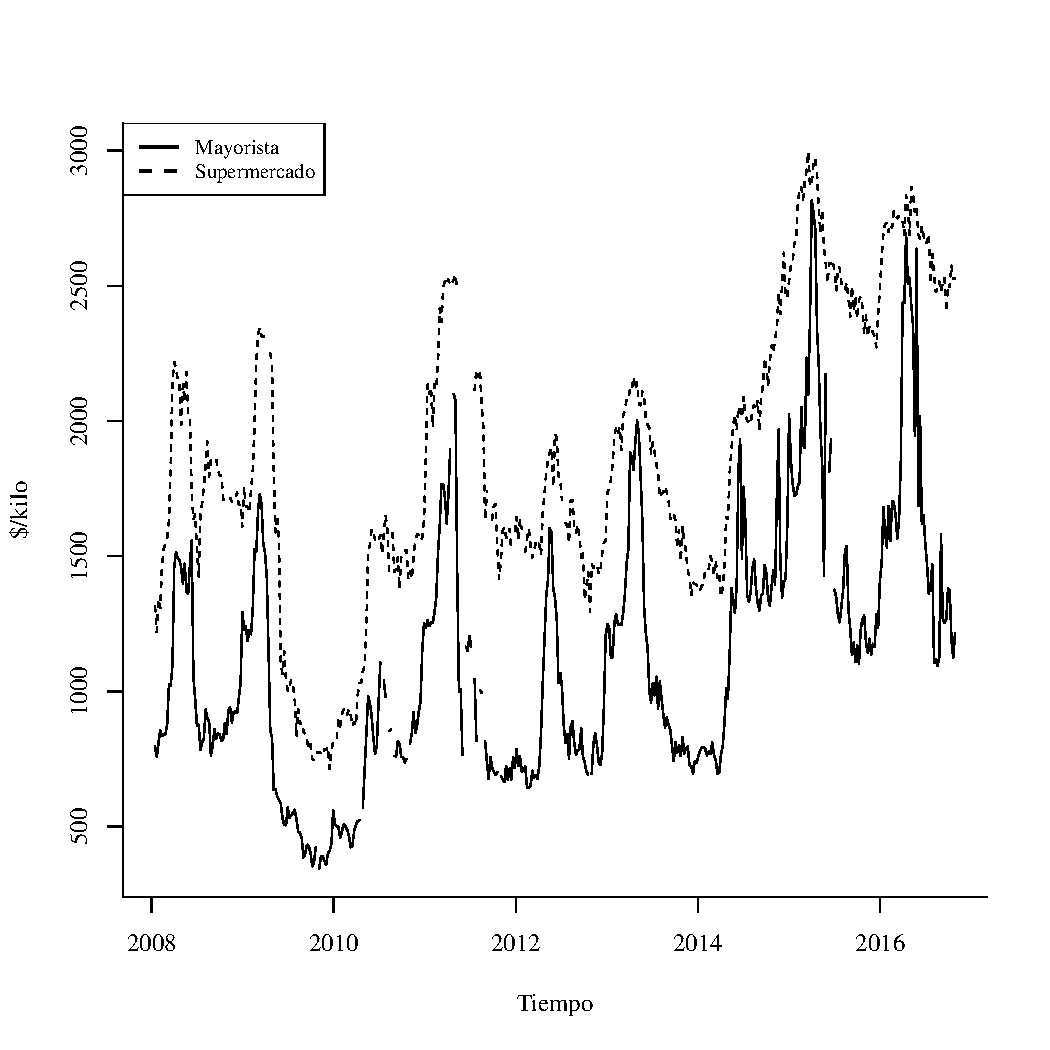
\includegraphics[width=6.5in,height=3.5in]{figure/fig-1-1} 

}

\caption[Evolución de precios del palta de larga vida de primera calidad,2008-2016]{Evolución de precios del palta de larga vida de primera calidad,2008-2016}\label{fig:fig-1}
\end{figure}


\end{knitrout}


\begin{knitrout}
\definecolor{shadecolor}{rgb}{0.969, 0.969, 0.969}\color{fgcolor}\begin{figure}[H]

{\centering 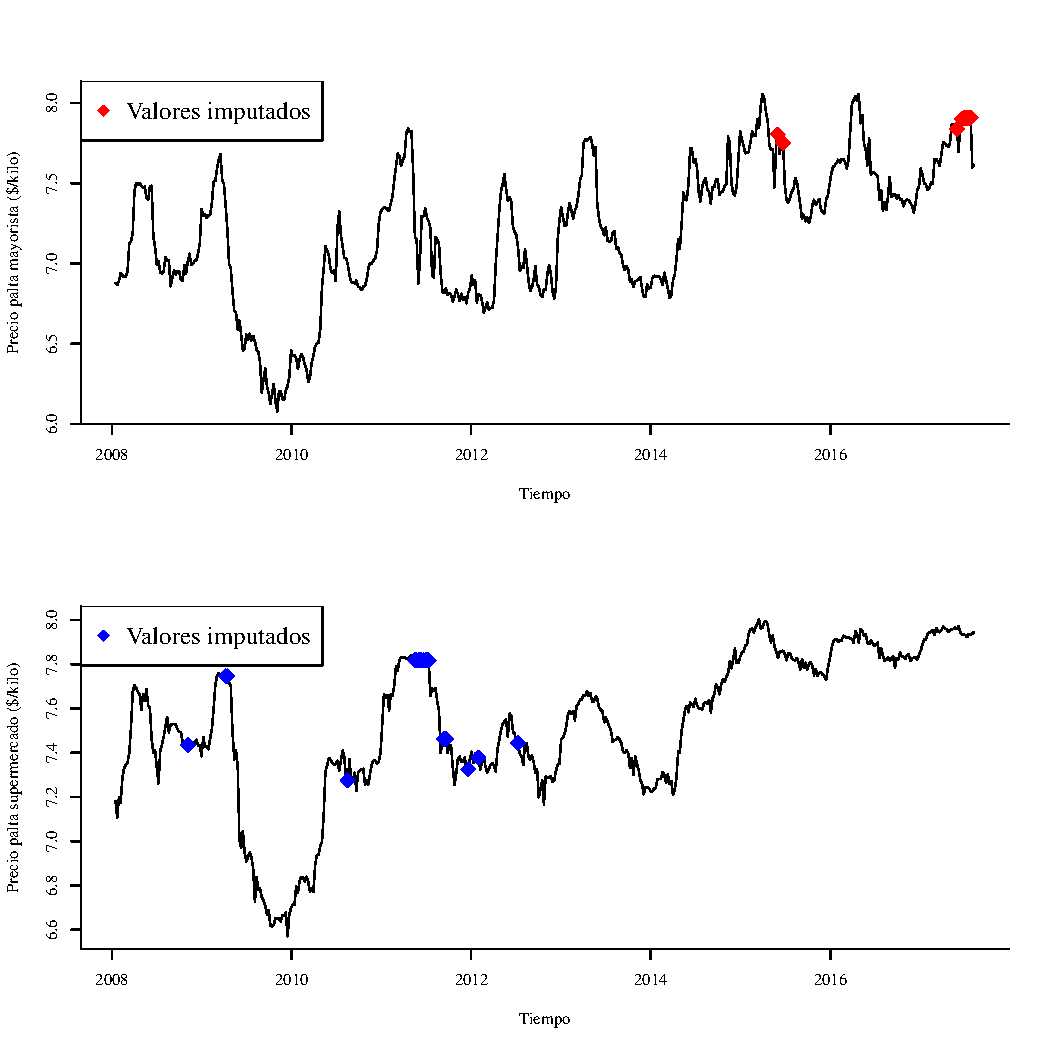
\includegraphics[width=6.5in,height=4.5in]{figure/fig-2-1} 

}

\caption[Imputación de valores perdidos a través del filtro de Kalman]{Imputación de valores perdidos a través del filtro de Kalman}\label{fig:fig-2}
\end{figure}


\end{knitrout}


\section{Análisis del orden de integración de las series}
\subsection{Análisis gráfico}

\begin{knitrout}
\definecolor{shadecolor}{rgb}{0.969, 0.969, 0.969}\color{fgcolor}\begin{figure}[H]

{\centering 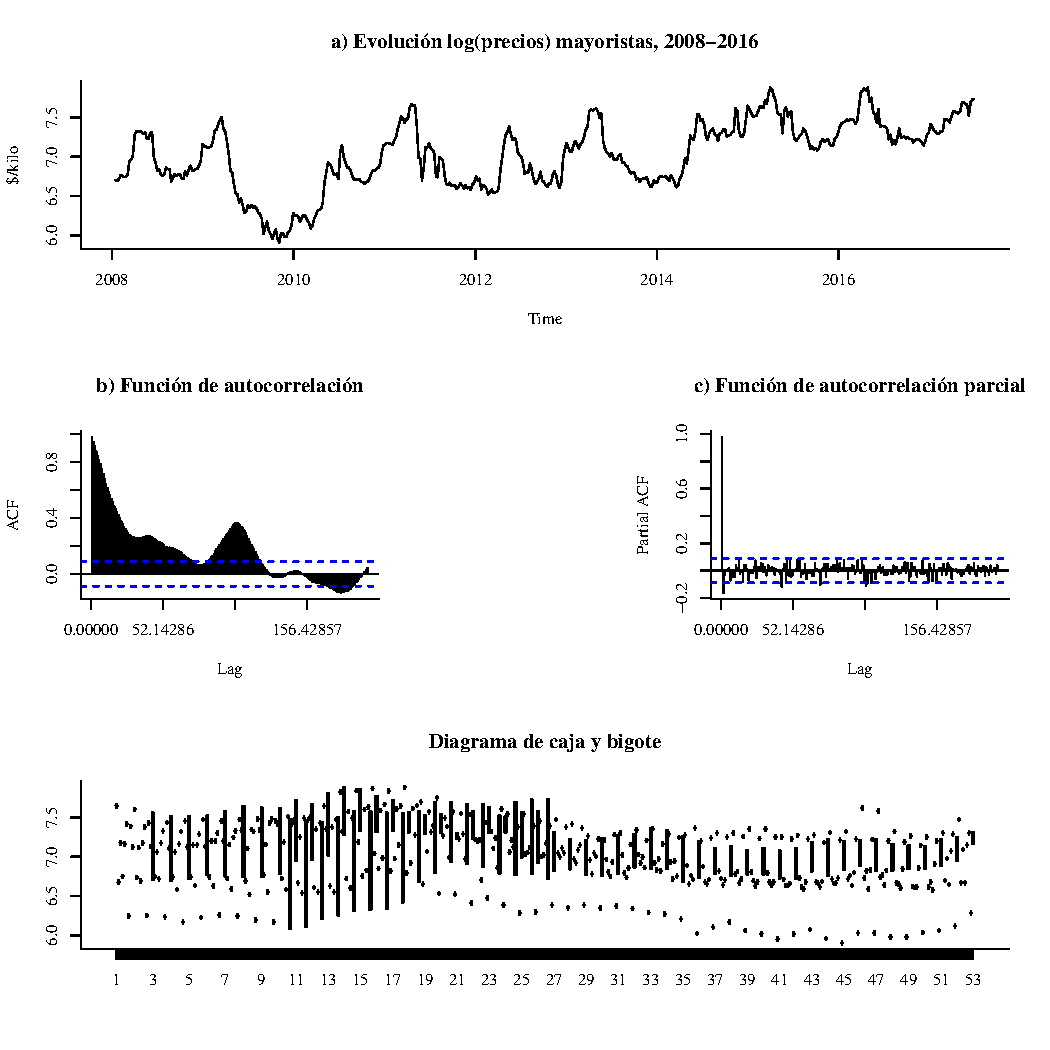
\includegraphics[width=6in,height=6.5in]{figure/fig-2_1-1} 

}

\caption[Evolución del logaritmo del precio mayorista de la palta ,2008-2016]{Evolución del logaritmo del precio mayorista de la palta ,2008-2016}\label{fig:fig-2.1}
\end{figure}


\end{knitrout}


\begin{knitrout}
\definecolor{shadecolor}{rgb}{0.969, 0.969, 0.969}\color{fgcolor}\begin{figure}[H]

{\centering 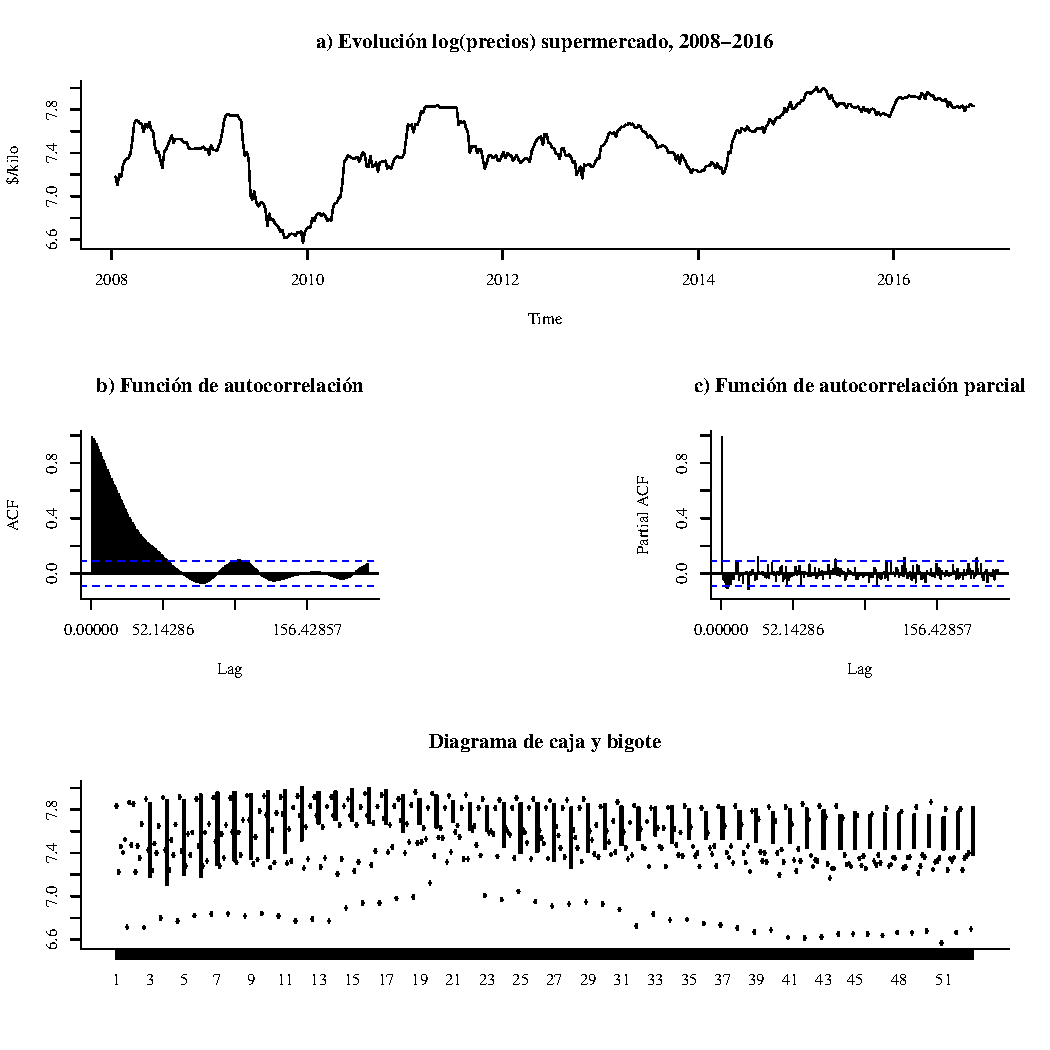
\includegraphics[width=6in,height=6.5in]{figure/fig-2_2-1} 

}

\caption[Evolución del logaritmo del precio en supermercado de la palta ,2008-2016]{Evolución del logaritmo del precio en supermercado de la palta ,2008-2016}\label{fig:fig-2.2}
\end{figure}


\end{knitrout}

\section{Contrastes de raíz unitaria}
\subsection{Contraste de Dickey-Fuller Aumentado}

El contraste más utilizado en la investigación aplicada, dada su simplicidad, es el contraste propuesto por \cite{fuller1976} y \cite{dickey1981}. Para aplicar este contraste existen dos posibles modelos 

Si $y_{t}$ satisface la siguiente ecuación

\begin{equation}
y_{t} = \alpha+\rho y_{t-1}+\epsilon_{t}\qquad (t=1,...,n)
\end{equation}
Donde $\epsilon_{t}\sim \mathcal{N}(0,\sigma^{2})$. 

Si $y_{t}$ satisface la siguiente ecuación 

Como puede observarse en el cuadro \ref{tab-1}, existen 3 estadísticos, $\Phi_{1},\quad \Phi_{2}$ y $\Phi_{3}$, y sus respectivas hipótesis que pueden ser utilizados. Mientras $\Phi_{1}$
\begin{equation}
y_{t} = \alpha+\beta\left(t-1-\frac{1}{2}n\right)+\rho y_{t-1}+\epsilon_{t}\qquad (t=1,...,n)
\end{equation}
Donde $\epsilon_{t}\sim \mathcal{N}(0,\sigma^{2})$. 

\begin{table}[h]
\centering
\begin{threeparttable}
\caption{Hipótesis del contraste de Dickey-Fuller}
\begin{tabular}{@{}llrllll@{}}
\toprule
\multicolumn{2}{l}{Estadístico} & \multicolumn{2}{c}{$\mathcal{H}_{0}$} &
\multicolumn{2}{c}{$\mathcal{H}_{a}$} \\
\cmidrule(l){3-4} \cmidrule(l){5-6} \\
\multicolumn{2}{l}{$\Phi_{1}$} &
\multicolumn{2}{l}{$(\alpha,\rho)=(0,1)$} &
\multicolumn{2}{l}{$(\alpha,\rho)\neq(0,1)$} \\
\multicolumn{2}{l}{$\Phi_{2}$} &
\multicolumn{2}{l}{$(\alpha,\beta, \rho)=(0,0,1)$} &
\multicolumn{2}{l}{$(\alpha,\beta,\rho)\neq(0,0,1)$} \\
\multicolumn{2}{l}{$\Phi_{3}$} &
\multicolumn{2}{l}{$(\alpha,\beta, \rho)=(\alpha,0,1)$} &
\multicolumn{2}{l}{$(\alpha,\beta,\rho)\neq(\alpha,0,1)$} \\
\bottomrule
\end{tabular}
\label{tab-1}
\begin{tablenotes}
\small
\item Fuente: Elaboración propia basado en Dickey y Fuller (1981)
\end{tablenotes}
\end{threeparttable}
\end{table}

\subsection{Contraste de Phillips Perron (1992)}

De manera similar al contraste anterior \cite{phillips1988} proponen 
\subsection{Contraste Kiatkowsky, Pesaran, Schmidt \& Shin (1992)}
\subsection{Contraste de Elliot, Rothenberg \& Stock (1993)} 

\subsection{Contraste de Canova \& Hansen (1995) para estacionalidad estable}

\section{Resultados de los contrastes de raíz unitaria}




\begin{table}[H]
\centering
\begin{threeparttable}
\caption{Contraste de Dickey-Fuller aumentado (con tendencia determinista)}
\begin{tabular}{@{}lrllll@{}}
\toprule
\multicolumn{1}{l}{} & \multicolumn{2}{c}{Estadístico} &
\multicolumn{3}{c}{Valores críticos} \\
\cmidrule(l){2-3} \cmidrule(l){4-6} \\
\multicolumn{1}{l}{$\mathcal{H}_0$} & \multicolumn{1}{c}{Mayorista$^{a}$} &
 \multicolumn{1}{c}{Supermercado$^{b}$} &
\multicolumn{1}{l}{90\%}&
\multicolumn{1}{l}{95\%}&
\multicolumn{1}{l}{99\%}
\\
\midrule
$\tau_{3} $  & -3.1822 &  -2.0437 & -3.13 & -3.42 & -3.98 \\
$\phi_{2} $  & 3.393   &  1.5448 & 4.05 & 4.71 & 6.15 \\
$\phi_{3}$   & 5.0686  &  2.0907 &    5.36    &   6.30   &  8.34    \\ 
\bottomrule
\end{tabular}
\label{tab-2}
\begin{tablenotes}
\small 
\item $^{a}$: Con un rezago, de acuerdo a criterio BIC. 
\item $^{b}$: Con un rezago, de acuerdo a criterio BIC. 
\end{tablenotes}
\end{threeparttable}
\end{table}

\begin{table}[H]
\centering
\begin{threeparttable}
\caption{Contraste de Dickey-Fuller aumentado (con drift)}
\begin{tabular}{@{}lrllll@{}}
\toprule
\multicolumn{1}{l}{} & \multicolumn{2}{c}{Estadístico} &
\multicolumn{3}{c}{Valores críticos} \\
\cmidrule(l){2-3} \cmidrule(l){4-6} \\
\multicolumn{1}{l}{$\mathcal{H}_0$} & \multicolumn{1}{c}{Mayorista$^{a}$} &
 \multicolumn{1}{c}{Supermercado$^{b}$} &
\multicolumn{1}{l}{90\%}&
\multicolumn{1}{l}{95\%}&
\multicolumn{1}{l}{99\%}
\\
\midrule
$\tau_{2} $  & -2.7628 &  -1.7114 & -2.57 & -2.87 & -3.44 \\
$\phi_{1} $  & 3.8373  &  1.6909 & 1.6909 & 4.61 & 3.79 \\
\bottomrule
\end{tabular}
\label{tab-3}
\begin{tablenotes}
\small 
\item $^{a}$: Con un rezago, de acuerdo a criterio BIC. 
\item $^{b}$: Con un rezago, de acuerdo a criterio BIC. 
\end{tablenotes}
\end{threeparttable}
\end{table}



\begin{table}[H]
\centering
\begin{threeparttable}
\caption{Contraste Phillips \& Perron$^{a}$ (con tendencia determinista)}
\begin{tabular}{@{}lrll@{}}
\toprule

 & \multicolumn{1}{c}{$Z-\alpha$} &
\multicolumn{1}{l}{$Z-\tau-\mu$}&
\multicolumn{1}{l}{$Z-\tau-\beta$}
\\
\cmidrule(l){2-2} \cmidrule(l){3-4} \\
Mayorista  & -22.122 &  2.1588 & 1.7097\\
Supermercado & -11.1245 & 1.0301 & 1.4522 \\
\bottomrule
\end{tabular}
\label{tab-4}
\begin{tablenotes}
\small 
\item $^{a}$: Con cinco rezagos de acuerdo a la siguiente regla $\root 4 \of {4 \times (n/100)}$. 
\end{tablenotes}
\end{threeparttable}
\end{table}





\begin{table}[H]
\centering
\begin{threeparttable}
\caption{Contraste Phillips \& Perron$^{a}$ (con tendencia determinista)}
\begin{tabular}{@{}lrl@{}}
\toprule

 & \multicolumn{1}{c}{$Z-\alpha$} &
\multicolumn{1}{l}{$Z-\tau-\mu$}
\\
\cmidrule(l){2-2} \cmidrule(l){3-3} \\
Mayorista  & -16.0952 &  2.8635 \\
Supermercado & -7.2938 & 1.9177 \\
\bottomrule
\end{tabular}
\label{tab-5}
\begin{tablenotes}
\small 
\item $^{a}$: Con cinco rezagos de acuerdo a la siguiente regla $\root 4 \of {4 \times (n/100)}$. 
\end{tablenotes}
\end{threeparttable}
\end{table}



\begin{table}[H]
\centering
\begin{threeparttable}
\caption{Contraste KPSS (con tendencia determinista)}
\begin{tabular}{@{}lrllll@{}}
\toprule
\multicolumn{1}{l}{} & \multicolumn{2}{c}{Estadístico} &
\multicolumn{3}{c}{Valores críticos} \\
\cmidrule(l){2-3} \cmidrule(l){4-6} \\
\multicolumn{1}{l}{$\mathcal{H}_0$} & \multicolumn{1}{c}{Mayorista$^{a}$} &
 \multicolumn{1}{c}{Supermercado$^{b}$} &
\multicolumn{1}{l}{90\%}&
\multicolumn{1}{l}{95\%}&
\multicolumn{1}{l}{99\%}
\\
\midrule
$\tau_{3} $  & 0.2657 &  0.3246 & 0.119 & 0.146 & 0.216 \\
\bottomrule
\end{tabular}
\label{tab-6}
\begin{tablenotes}
\small 
\item $^{a}$: Con cinco rezagos de acuerdo a la siguiente regla $\root 4 \of {4 \times (n/100)}$. 
\item $^{b}$: Con cinco rezagos de acuerdo a la siguiente regla $\root 4 \of {4 \times (n/100)}$. 
\end{tablenotes}
\end{threeparttable}
\end{table}


\begin{table}[H]
\centering
\begin{threeparttable}
\caption{Contraste KPSS (sin tendencia determinista)}
\begin{tabular}{@{}lrllll@{}}
\toprule
\multicolumn{1}{l}{} & \multicolumn{2}{c}{Estadístico} &
\multicolumn{3}{c}{Valores críticos} \\
\cmidrule(l){2-3} \cmidrule(l){4-6} \\
\multicolumn{1}{l}{$\mathcal{H}_0$} & \multicolumn{1}{c}{Mayorista$^{a}$} &
 \multicolumn{1}{c}{Supermercado$^{b}$} &
\multicolumn{1}{l}{90\%}&
\multicolumn{1}{l}{95\%}&
\multicolumn{1}{l}{99\%}
\\
\midrule
$\tau_{3} $  & 2.5592 &  2.9497 & 0.347 & 0.463 & 0.739 \\
\bottomrule
\end{tabular}
\label{tab-7}
\begin{tablenotes}
\small 
\item $^{a}$: Con cinco rezagos de acuerdo a la siguiente regla $\root 4 \of {4 \times (n/100)}$. 
\item $^{b}$: Con cinco rezagos de acuerdo a la siguiente regla $\root 4 \of {4 \times (n/100)}$. 
\end{tablenotes}
\end{threeparttable}
\end{table}





\begin{table}[H]
\centering
\begin{threeparttable}
\caption{Contraste de Elliot, Rothenberg \& Stock (con tendencia determinista)}
\begin{tabular}{@{}lrllll@{}}
\toprule
\multicolumn{1}{l}{} & \multicolumn{2}{c}{Estadístico} &
\multicolumn{3}{c}{Valores críticos} \\
\cmidrule(l){2-3} \cmidrule(l){4-6} \\
\multicolumn{1}{l}{} & \multicolumn{1}{c}{Mayorista$^{a}$} &
 \multicolumn{1}{c}{Supermercado$^{b}$} &
\multicolumn{1}{l}{90\%}&
\multicolumn{1}{l}{95\%}&
\multicolumn{1}{l}{99\%}
\\
\midrule
  & -3.1558 &  -2.0504 & -2.57 & -2.89 & -3.48 \\
\bottomrule
\end{tabular}
\label{tab-8}
\begin{tablenotes}
\small 
\item $^{a}$: Con un rezago, de acuerdo a criterio BIC. 
\item $^{b}$: Con un rezago, de acuerdo a criterio BIC. 
\end{tablenotes}
\end{threeparttable}
\end{table}

\begin{table}[H]
\centering
\begin{threeparttable}
\caption{Contraste de Elliot, Rothenberg \& Stock (con constante)}
\begin{tabular}{@{}lrllll@{}}
\toprule
\multicolumn{1}{l}{} & \multicolumn{2}{c}{Estadístico} &
\multicolumn{3}{c}{Valores críticos} \\
\cmidrule(l){2-3} \cmidrule(l){4-6} \\
\multicolumn{1}{l}{} & \multicolumn{1}{c}{Mayorista$^{a}$} &
 \multicolumn{1}{c}{Supermercado$^{b}$} &
\multicolumn{1}{l}{90\%}&
\multicolumn{1}{l}{95\%}&
\multicolumn{1}{l}{99\%}
\\
\midrule
  & -2.3519 &  -0.8837 & -1.62 & -1.94 & -2.57 \\
\bottomrule
\end{tabular}
\label{tab-9}
\begin{tablenotes}
\small 
\item $^{a}$: Con un rezago, de acuerdo a criterio BIC. 
\item $^{b}$: Con un rezago, de acuerdo a criterio BIC. 
\end{tablenotes}
\end{threeparttable}
\end{table}




\begin{table}[H]
\centering
\caption{Contraste de Canova \& Hansen$^{a}$}
\begin{threeparttable}
\begin{tabular}{@{}lll@{}}
\toprule 
	&	Estadístico	&	valor-p	\\
\cmidrule(l){2-2} \cmidrule(l){3-3} \\	
$	2\pi/52.14	$	& 	0.227	& 	0.6999	\\
$	4\pi/52.14	$	&	0.2603	&	0.6133	\\
$	6\pi/52.14	$	& 	0.32	& 	0.4755	\\
$	8\pi/52.14	$	&	0.2532	&	0.6312	\\
$	10\pi/52.14	$	& 	0.3436	& 	0.4287	\\
$	12\pi/52.14	$	&	0.2876	&	0.547	\\
$	14\pi/52.14	$	& 	0.2109	& 	0.7432	\\
$	16\pi/52.14	$	&	0.2976	&	0.5239	\\
$	18\pi/52.14	$	& 	0.2948	& 	0.5304	\\
$	20\pi/52.14	$	&	0.383	&	0.3595	\\
$	22\pi/52.14	$	& 	0.306	& 	0.5052	\\
$	24\pi/52.14	$	&	0.3091	&	0.4985	\\
$	26\pi/52.14	$	& 	0.2195	& 	0.7199	\\
$	28\pi/52.14	$	&	0.4032	&	0.3282	\\
$	30\pi/52.14	$	& 	0.3891	& 	0.3498	\\
$	32\pi/52.14	$	&	0.1906	&	0.7979	\\
$	34\pi/52.14	$	& 	0.2511	& 	0.6367	\\
$	36\pi/52.14	$	&	0.2742	&	0.5789	\\
$	38\pi/52.14	$	& 	0.6599	& 	0.0982	\\
$	40\pi/52.14	$	&	0.2673	&	0.5959	\\
$	42\pi/52.14	$	& 	0.2401	& 	0.6652	\\
$	44\pi/52.14	$	&	0.1919	&	0.7945	\\
$	46\pi/52.14	$	& 	0.5093	& 	0.2012	\\
$	48\pi/52.14	$	&	0.303	&	0.5119	\\
$	50\pi/52.14	$	& 	0.2531	& 	0.6314	\\
$	52\pi/52.14	$	&	0.476	&	0.235	\\
$	joint	$	& 	5.1191	& 	1	\\
\bottomrule 
\end{tabular}
\begin{tablenotes}
\small
\item $^{a}$: El contraste utiliza términos trigonométricos
\end{tablenotes}
\end{threeparttable}
\end{table}

\chapter{Análisis de cointegración}
\section{Cointegración y análisis de las relaciones de largo plazo}

{\color{red} \textbf{Apuntes de Juselius}

\begin{itemize}
\item The time series describing cumulated trend-adjusted shocks is usually called a stochas-
tic trend. It is a cumulation of random shocks with zero mean and constant variance. If
\item with a linear deterministic trend component. Thus, the difference between a stochastic
and deterministic trend is that the increments of a stochastic trend change randomly,
whereas those of a deterministic trend are constant over time.
\item It is easy to see that if inflation rate is I(1) with a non-zero mean, then prices will contain
a integrated twice cumulated of order stochastic two, or in trend, 
t
 s=1 notation
i=1 s
 εi . pt We ∼ say I(2).
 that trend-adjusted prices are
\item We shall argue below that, unless a unit root is given a structural interpretation, the
choice of one representation or the other is as such not very important, as long as there is
consistency between the economic analysis and the choice. However, from an econometric
point of view the choice between the two representations is usually crucial for the whole
empirical analysis and should therefore be carefully considered.
\item variable.
Because a cointegrating relation does not necessarily correspond to an interpretable
economic relation, we make a further distinction between the statistical concept of a
‘cointegration relation’ and the economic concept of a ‘long-run equilibrium relation’.
\item say second that stochastic the distinction trend,
 between 
 u2i , as a long-run a long-run and structural medium-run trend stochastic or not. trend Thus,in one this might
 case
is between an I(1) stochastic trend with no linear trend and a near I(1) stochastic trend
with a linear trend.

\end{itemize}

\begin{defin}
Sea $\{\bold{x}_{t}\}$ un proceso estocástico para $t=..., -1,0,1,2,...$ Si 

\begin{align}
\mathbb{E}[\bold{x}_{t}] & =-\infty < \bold{\mu} <\infty \\ 
\mathbb{E}[\bold{x}_{t}-\bold{\mu}]^{2} & = \bold{\Sigma}_{0}<\infty \qquad \forall t\\ 
\mathbb{E}[(\bold{x}_{t}-\bold{\mu})(\bold{x}_{t+h}-\bold{\mu})] & = \bold{\Sigma}_{h} \qquad \forall \text{t y h}
\end{align}
Entonces $\bold{x}_{t}$ es \textit{debilmente estacionario}. La estacionariedad estricta requiere que la distribución de $(x_{t1},...,x_{tk})$ es la misma que $(x_{t1+h},...,x_{tk+h})$ para $h=...,-1,0,1,2,...$
\end{defin}

for time t based on the available information at time t − 1. For example, a VAR model
with autocorrelated and or heteroscedastic residuals would describe agents that do not
use all information in the data as efficiently as possible. This is because by including the

 For example, a VAR model
with autocorrelated and or heteroscedastic residuals would describe agents that do not
use all information in the data as efficiently as possible. 

Simulation studies have shown that valid statistical inference is sensitive to violation
of some of the assumptions, such as parameter non-constancy, autocorrelated residu-
als (the higher, the worse) and skewed residuals, while quite robust to others, such as
excess kurtosis and residual heteroscedasticity. This will be discussed in more detail in


• the use of intervention dummies to account for significant political or institutional
events during the sample;
• conditioning on weakly or strongly exogenous variables;
• checking the measurements of the chosen variables;
• changing the sample period to avoid fundamental regime shift or splitting the sample
into more homogenous periods.

and the model has been extended to contain Dt , a vector of deterministic components,
such as a constant, seasonal dummies and intervention dummies. The autoregressive for-
mulation is useful for expressing hypotheses on economic behaviour, whereas the moving average representation is useful when examining the properties of the proces.

Si asumimos un modelo $VAR(2)$ bi-dimensional

\begin{equation}
(\bold{I}-\boldsymbol{\Pi}_{1}L-\boldsymbol{\Pi}_{2}L^{2})\bold{x}_{t} = \boldsymbol{\Phi}\bold{D}_{t}+\bold{\varepsilon}_{t}
\end{equation}

La función características es entonces 

\begin{align}
\bold{\Pi}(z) & = \bold{I}-\left[\begin{array}{cc} 
\pi_{1.11} & \pi_{1.12} \\
\pi_{1.21} & \pi_{1.22}
\end{array}\right]z- \left[\begin{array}{cc} 
\pi_{2.11} & \pi_{2.12} \\
\pi_{2.21} & \pi_{2.22}
\end{array}\right]z^{2} \\
              & = \bold{I}-\left[\begin{array}{cc} 
\pi_{1.11}z & \pi_{1.12}z \\
\pi_{1.21}z & \pi_{1.22}z
\end{array}\right]- \left[\begin{array}{cc} 
\pi_{2.11}z^{2} & \pi_{2.12}z^{2} \\
\pi_{2.21}z^{2} & \pi_{2.22}z^{2}
\end{array}\right] \\
 & = \left[\begin{array}{cc} (1-\pi_{1.11}z-\pi_{2.11}z^{2}) & (-\pi_{1.12}z-\pi_{2.12}z^{2}) \\ 
 (-\pi_{1.21}z-\pi_{2.21}z^{2}) & (1-\pi_{1.22}z-\pi_{2.22}z^{2})
 \end{array}\right]
\end{align}
y 

\begin{align}
|\boldsymbol{\Pi}(z)| & = (1-\pi_{1.11}z-\pi_{2.11}z^{2})(1-\pi_{1.22}z-\pi_{2.22}z^{2})-(\pi_{1.12}z+\pi_{2.12}z^{2})(\pi_{1.21}z+\pi_{2.21}z^{2}) \\ 
& = 1-a_{1}z-a_{2}z^{2}-a_{3}z^{3}-a_{4}z^{4} \\ 
& = (1-\rho_{1}z)(1-\rho_{2}z)(1-\rho_{3}z)(1-\rho_{4}z)
\end{align}

El determinante entrega información valiosa sobre el comportamiento dinámico del proceso. 

Luego 

\begin{align}
\bold{x}_{t} & = \frac{\boldsymbol{\Pi}^{a}(L)(\boldsymbol{\Phi}\bold{D}_{t}+\varepsilon_{t})}{(1-\rho_{1}z)(1-\rho_{2}z)(1-\rho_{3}z)(1-\rho_{4}z)}+\tilde{\bold{X}}^{0}, \qquad t=1,...,T \\ 
& = \left(\frac{\bold{\Pi}_{1}^{a}L+\bold{\Pi}^{a}_{2}L^{2}}{(1-\rho_{2}z)(1-\rho_{3}z)(1-\rho_{4}z)}\right)\left(\frac{\varepsilon_{t}+\bold{\Phi}D_{t}}{(1-\rho_{1}L)}\right)+\bold{\tild{X}}^{0}, \qquad t=1,...,T
\end{align}

\section{Estimación basada en la verosimilitud para el modelo VAR irrestricto}

Cuando el modelo no tiene restricciones sobre sus parámetros (como las que pueden surgir debido a la presencia de raíces unitarias) el modelo puede estimarse por MCO, caso que coincide con el estimador de \textit{Full information maximum likelihood}

Si escribimos el modelo en su versión apilada
\begin{align}
& \bold{x}_{t} = \bold{B'Z}_{t}+\varepsilon_{t}, \qquad t=1,..,T \\ 
& \varepsilon_{t}\sim IN_{p}(\bold{0,\Omega})
\end{align}

Donde: 
\begin{itemize}
\item $\bold{B'}=\left[\boldsymbol{\mu_{0}, \Pi_{1}, \Pi_{2},...,\Pi_{k}}\right]$
\item $\bold{Z'}_{t} = \left[\bold{1,x'_{t-1}, x'_{t-2},...,x'_{t-k}}\right]$
\item $\bold{X}^{0}$ = \left[\bold{x'_{0}, x'_{-1},...,x'_{-k+1}}\right]$ 
\end{itemize}

La función de verosimilitud será la siguiente: 

\begin{equation}
\log L(\boldsymbol{B,\Omega,X}) = -T\frac{p}{2}\log(2\pi)-T\frac{1}{2}\log|\bold{\Omega}|-\frac{1}{2}\sum_{t=1}^{T}(\bold{x_{t}-B'Z_{t}})'\boldsymbol{\Omega}^{-1}(\bold{x_{t}-B'Z_{t}})
\end{equation}

Si calculamos $\frac{\partial \log L}{\partial \bold{B}}$, tendremos
\begin{equation*}
\sum_{t=1}^{T}\bold{x_{t}Z'_{t}} = \bold{\tilde{B}'}\sum_{t=1}^{T}\bold{Z_{t}Z_{t}'}
\end{equation*}

Entonces, el estimador de máxima verosimilitud es 

\begin{equation}
\bold{\tilde{B}}' = \sum_{t=1}^{T}(\bold{x_{t}Z'_{t}})\left(\sum_{t=1}^{T}\bold{Z_{t}Z'_{t}}\right)^{-1} = \bold{M}_{xZ}\bold{M}_{ZZ}^{-1}
\end{equation}

Luego calculando $\frac{\partial \log L}{\partial \boldsymbol{\Omega}}=\bold{0}$

\begin{equation}
\boldsymbol{\hat{\Omega}} = T^{-1}\sum_{t=1}^{T}(\bold{x_{t}-\hat{B}'Z_{t}})(\bold{x_{t}-\hat{B}'Z_{t}})' = T^{-1}\sum_{t=1}^{T}\boldsymbol{\hat{\varepsilon}_{t}\hat{\varepsilon}'_{t}}
\end{equation}

El valor máximo de la función de Verosimilitud, será el siguiente: 

\begin{equation}
\log L _{\max} = -\frac{P}{2}T\log (2\pi)-\frac{1}{2}T\log|\boldsymbol{\hat{\Omega}}|-\frac{1}{2}\sum_{t=1}^{T}(\bold{x_{t}-\hat{B}'Z_{t}})'\boldsymbol{\hat{\Omega}}^{-1}(\bold{x_{t}-\hat{B}'Z_{t}}) 
\end{equation}

Mostraremos que $\log L_{\max} = -\frac{1}{2}T\log |\boldsymbol{\hat{\Omega}}|+K, \qquad K\in \mathbb{R}$

\begin{align}
(\boldsymbol{x_{t}-\hat{B}'Z_{t}})\boldsymbol{\hat{\Omega}}^{-1}(\bold{x_{t}-\hat{B}'Z_{t}}) 
& = \boldsymbol{\hat{\varepsilon}'_{t}\boldsymbol{\hat{\Omega}}^{-1}\hat{\varepsilon}_{t}} \nonumber \\
& = \sum_{ij}\hat{\varepsilon}_{t,i}(\boldsymbol{\hat{\Omega}}^{-1})_{ij}\hat{\varepsilon}_{t,j} \\
& = \sum_{ij}(\boldsymbol{\hat{\Omega}}^{-1})_{ij}\hat{\varepsilon}_{t,i}\hat{\varepsilon}_{t,j} \nonumber \\ 
& = \text{traza}\{\boldsymbol{\hat{\Omega}}^{-1}\boldsymbol{\hat{\varepsilon_{t}}\hat{\varepsilon}'_{t}}\}
\end{align}

Luego, se tiene que 

\begin{align}
\sum_{t=1}^{T}(\bold{x_{t}-\hat{B}'Z_{t}})\boldsymbol{\hat{\Omega}}^{-1}(\bold{x_{t}-\hat{B}'Z_{t}})' & = \sum_{t=1}^{T}\text{traza}\{\boldsymbol{\hat{\Omega}}^{-1}\boldsymbol{\hat{\varepsilon_{t}}\hat{\varepsilon}'_{t}}\} \\
& = T \sum_{t=1}^{T}\text{traza}\{\boldsymbol{\hat{\Omega}}^{-1}\boldsymbol{\hat{\varepsilon_{t}}\hat{\varepsilon}'_{t}}/T\} \\ 
& = T \text{traza}\{\boldsymbol{\hat{\Omega}}^{-1}\hat{\Omega}\} \\ 
& = T \text{traza}\{\bold{I}_{p}\} = Tp
\end{align}

De donde se desprende que 

\begin{equation}
\log L_{\max} = -T \frac{1}{2} \log |\boldsymbol{\hat{\Omega}}|\underbrace{-T\frac{p}{2}-T\frac{p}{2}\log(2\pi)}_{+K}
\end{equation}

\textbf{NOTA PARA RECORDAR: si las variables del modelo están formuladas en logaritmo la desviación estándar de cada una de estas puede ser interpretada como un porcentaje de error }


\subsection{Contraste de razón de verosimilitud}

\begin{equation}
  -2\log Q(\mathcal{H}_{k}/\mathcal{H}_{k+1}) =  T(\log|\boldsymbol{\hat{\Omega}}_{k}|-\log|\boldsymbol{\hat{\Omega}}_{k+1}|) \sim \chi^{2}_{p^{2}}
\end{equation}


Criterios de selección 

\begin{align}
\text{AIC} & = \log |\boldsymbol{\hat{\Omega}}|+(p^{2}k)\frac{2}{T} \\ 
\text{SC} & = \log|\boldsymbol{\hat{\Omega}}|+(p^{2}k)\frac{\log T}{T} \\ 
\text{Hannah-Quinn} & = \log|\boldsymbol{\hat{\Omega}}|+(p^{2}k)\frac{2\log \log T}{T}
\end{align}

Todos los criterios en común están basados en el máximo valor que alcanza la función de verosimilitud del modelo, más un factor que penaliza por el número de parámetros estimados. 

\textbf{
Al momento de la determinación del número de rezagos, volver a revisar tabla 4.5 de la página 92}

\begin{equation}
\text{Trace correlation} = 1-\text{traza}(\boldsymbol{\hat{\Omega}}[\text{Cov}(\bold{\Delta x_{t}})]^{-1})/p 
\end{equation}


\subsubsection{El contraste de Ljung-Box}

\begin{equation}
\text{Ljung-Box} = T(T+2)\sum_{h=1}^{T/4}(T-h)^{-1}\text{traza}(\boldsymbol{\hat{\Omega}'_{h}\hat{\Omega}^{-1}\hat{\Omega}'_{h}\hat{\Omega}^{-1}})
\end{equation}

Donde  $ \boldsymbol{\hat{\Omega}}_{h} = T^{-1}\sum_{t=1}^{T}\boldsymbol{\hat{\varepsilon}_{t}\hat{\varepsilon}_{t-h}'}$. El estadístico se considera distribuido aproximadamente según una $\chi^{2}$ con $p^{2}(T/4-k+1)-p^{2}$ grados de libertad. 

También puede utilizarse un contraste propuesto por Godfrey(1988),  el cual consiste en regresar los residuos del modelo VAR estimado, $\boldsymbol{\hat{\varepsilon}_{t}}$, sobre $k$ variables rezagadas, $\bold{x_{t-1}, x_{t-2}, ...,x_{t-k}}$ y el $j$-ésimo residuo rezagado

\begin{equation}
\boldsymbol{\hat{\varepsilon}_{t}}=\bold{A_{1}x_{t-1}+A_{2}x_{t-2}+...+A_{k}x_{t-k}+A_{\varepsilon}}\boldsymbol{\hat{\varepsilon}}
\end{equation}

}

\subsection{Modelo Vectorial de Corrección del Error (VECM)}
Suponga que  cada componente de una serie de tiempo $K$-dimensional $y_{t}$ es $I(1)$. Entonces, la ecuación (VAR) no será una formulación adecuada de este modelo debido a que los términos $y_{t},y_{t-1},...,y_{t-p}$ son todos no estacionarios. De todas formas, sustituyendo 
\begin{align}
\bf{A}_{1} & = \bf{I}_{k}+\bold{\Gamma}_{1} \\ 
\bf{A}_{i} & = \bold{\Gamma_{i}}-\bold{\Gamma_{i-1}} \qquad i=1,...,p-1 \\ 
\bf{A}_{p} & = -\bold{\Gamma}_{p-1}
\end{align}

En la ecuación (2.8), reagrupando términos y utilizando que $\Delta \bf{y}_{i} = \bf{y}_{i}-\bf{y}_{i-1}\quad \forall i$, podemos reescribir esta ecuación como 
\begin{equation}\label{vecm1}
\Delta \bf{y}_{t}=\bold{\mu}+\bold{\Gamma}_{1}\Delta \bf{y}_{t-1}+\bold{\Gamma}_{2}\Delta \bf{y}_{t-2}+...+\bold{\Gamma}_{p-1}\Delta \bf{y}_{t-p+1}+\bf{u}_{t}
\end{equation} 
Naturalmente, ambas ecuaciones describen el mismo modelo, pero preferimos usar la ecuación \eqref{vecm1} cuando $\bf{y}_{t}$ es $I(1)$, debido a que cada término es estacionario en este caso. Entonces, cuando $\bf{y}_{t}$ es $I(1)$, podemos encontrar un modelo apropiado para $y_{t}$ diferenciando cada componente de $\bf{y}_{t}$ una vez, y llevando a cabo la regresión basada en la ecuación \eqref{vecm1}. De todas formas, entonces no podremos tomar en cuenta que podría haber dependencias entre algunos de los componentes de $\bf{y}_{t}$. Por ejemplo, dos de los componentes podrían tener una tendencia en común, o podría existir una combinación lineal de los componente de $y_{t}$ la cual fuera estacionaria. Este problema suele resolverse utilizando incluyendo un \textbf{término de corrección del error} $\bold{\Pi}\bf{y}_{t-1}$ en la ecuación \eqref{vecm1}, donde $\bold{\Pi}$ es una matriz $K\times K$ de cuyo rango $rank(\bold{\Pi})<K$, debido a que si $\bold{\Pi}$ tuviera rango completo, entonces $\bold{\Pi}$  es invertible, de manera que la variable no estacionaria $\bf{y}_{t-1}$ puede ser escrita como la suma de términos estacionarios, lo que es una contradicción. Entonces, $rank(\bold{\Pi})=r<K$ lo cual implica que existen $(K\times r)-matrices$ $\boldsymbol{\alpha}$ y $\boldsymbol{\beta}$ de rango $r$ tales que $\bold{\Pi}=\boldsymbol{\alpha}\boldsymbol{\beta}'$. Entonces, cada una de las $r$ filas de $\boldsymbol{\beta}'\bf{y_{t-1}}$ es una combinación lineal estacionaria de los componentes de $y_{t}$ y es llamada una \textbf{relación de cointegración}. El número $r$, el cual es igual al número de relación de cointegración es llamado el \textbf{rango de cointegración}. Como la matriz $\boldsymbol{\beta}$ contiene todos los coeficiente de las relaciones de cointegración, es llamada \textbf{la matriz de cointegración}. La matriz $\boldsymbol{\alpha}$, la cual es la matriz de coeficientes de los términos estacionarios $\boldsymbol{\beta}'\bf{y_{t-1}}$ en la ecuación \eqref{vecm2}, es llamada la matriz de carga. 
\begin{defin}
Un modelo \textbf{VECM} de orden $p$ se define como 
\begin{equation}\label{vecm2}
\Delta \bf{y}_{t}=\boldsymbol{\mu}+\boldsymbol{\alpha\beta}'
\bf{y}_{t-1}+\bold{\Gamma}_{1}\Delta \bf{y}_{t-1}+...+\bold{\Gamma}_{p-1}\Delta \bf{y}_{t-p+1}+u_{t} \quad t=1,...,T
\end{equation}
Donde $\bf{y}_{t}=\left[y_{1t},...,y_{Kt}\right]'$ es un vector aleatorio de $K\times 1$, $\boldsymbol{\mu}$ es un vector constante de $(K\times 1)$, $\boldsymbol{\alpha}$ y $\boldsymbol{\beta}$ son matrices $(K\times r)$ tales que $rank(\boldsymbol{\alpha})=rank(\boldsymbol{\beta})<K$, 
\end{defin} 

\subsection{El contraste de cointegración de Johansen}

Considere el siguiente modelo 

\begin{equation}
\Delta \bf{y}_{t} = \Pi \bf{y}_{t-1}+\Gamma_{1}\Delta\bf{y}_{t-1}+...+\Gamma_{p-1}\Delta\bf{y}_{t-p+1}+u_{t}
\end{equation}

Donde $\bf{y}_{t}$ es un proceso $K$-dimensional y $rk(\Pi)=r$ con  $0\leq r\leq K$. 

\begin{align}
\mathcal{H}_{0}: rk(\bold{\Pi})=r_{0} && versus && \mathcal{H}_{1}: r_{0}< rk(\bold{\Pi}) \leq r_{1} \label{hipo_johansen1}
\end{align} 

Lütkepohl(2005, pp. 294)
Lütkepohl(2005, pp.340)
Tso (1981) Para regresión de rango reducido
\begin{teo}
Sea $M:=I_{T}-\Delta \bf{X}'(\Delta \bf{X}\Delta \bf{X}')^{-1}\Delta \bf{X}$, $R_{0}:=\Delta \bf{Y}M$ y $R_{1}=\bf{Y}_{-1}M$. Además 

\begin{equation}
S_{ij}:=R_{i}R'_{j}/T, \qquad i=0,1, 
\end{equation}
$\lambda_{1}\geq ... \geq \lambda_{K}$ los autovalores de $S_{11}^{-1/2}S_{10}S_{00}^{-1}S_{01}S_{11}^{-1/2}$, y $\bf{v}_{1},...,\bf{v}_{K}$, los correspondientes autovectores ortonormales 

\begin{align}
\log l  =  & -\frac{KT}{2}\log 2\pi-\frac{T}{2}\log |\bold{\Sigma}_{u}|  \nonumber \\ 
  & -\frac{1}{2}\text{tr}\left[(\Delta \bf{Y}-\boldsymbol{\alpha}\boldsymbol{\beta}'Y_{-1}-\bold{\Gamma}\Delta\bf{X})\bold{\Sigma_{u}}(\Delta \bf{Y}-\boldsymbol{\alpha}\boldsymbol{\beta}'Y_{-1}-\bold{\Gamma}\Delta\bf{X})\right] 
\end{align}
\end{teo}

Desde el resultado anterior puede plantearse el siguiente estadístico de razón de verosimilitud (LRT) para contrastar \eqref{hipo_johansen1}

\begin{align}
\lambda_{LR}(r_{0},r_{1}) & = 2[\log l(r_{1})-\log l(r_{0})] \nonumber \\ 
                          & = T\left[-\sum_{i=1}^{r_{1}}\log(1-\lambda_{i})+\sum_{i=1}^{r_{0}}\log(1-\lambda_{i})\right] \nonumber \\ 
                          & = -T\sum_{i=r_{0}+1}^{r_{1}}\log (1-\lambda_{i})
\end{align}
Cabe destacar que bajo la hipótesis nula, el estadístico no sigue una distribución estándar por lo que lo que sus valores críticos deben obtenerse mediante simulación. En particular, depende del número de relaciones de cointegracón y del tipo de hipótesis alterna a utilizar. Dos especificaciones son las más utilizadas en la literatura: 
\begin{align}
\mathcal{H}_{0}: rk(\bold{\Pi})=r_{0} &&  versus && \mathcal{H}_{1}: r_{0}<rk(\bold{\Pi})\leq K \label{hipo_johansen2}
\end{align}
y
\begin{align}
\mathcal{H}_{0}: rk(\bold{\Pi})=r_{0} &&  versus && \mathcal{H}_{1}: rk(\bold{\Pi})=r_{0}+1 \label{hipo_johansen3}
\end{align}
El estadístico $\lambda_{LR}(r_{0},K)$ para contrastar \eqref{hipo_johansen2} se denomina comunmente como el estadístico \textit{de la traza} para testear el rango de cointegración, mientras que $\lambda_{LR}(r_{0},r_{0}+1)$ es llamado estadístico de \textit{máximo autovalor}.  

\section{Resultados}
\subsection{Determinación del rango de cointegración}



\begin{knitrout}\scriptsize
\definecolor{shadecolor}{rgb}{0.969, 0.969, 0.969}\color{fgcolor}\begin{kframe}
\begin{verbatim}
## $L01
## [1] 8.792146
## 
## $df
## [1] 4
## 
## $`p-value`
## [1] 0.06651009
\end{verbatim}
\end{kframe}
\end{knitrout}


\begin{knitrout}
\definecolor{shadecolor}{rgb}{0.969, 0.969, 0.969}\color{fgcolor}\begin{kframe}
\begin{verbatim}
## #############
## ###Model VECM 
## #############
## Full sample size: 459 	End sample size: 456
## Number of variables: 2 	Number of estimated slope parameters 10
## AIC -4872.231 	BIC -4826.884 	SSR 5.736816
## Cointegrating vector (estimated by ML):
##    mayorista supermercado    const
## r1         1    -1.182243 1.932082
## 
## 
##                       ECT                mayorista -1      
## Equation mayorista    -0.1222(0.0278)*** 0.0719(0.0499)    
## Equation supermercado 0.0493(0.0130)***  0.0286(0.0234)    
##                       supermercado -1     mayorista -2     
## Equation mayorista    0.2706(0.0995)**    0.0958(0.0494).  
## Equation supermercado -0.0138(0.0466)     0.0528(0.0232)*  
##                       supermercado -2   
## Equation mayorista    0.1856(0.0994).   
## Equation supermercado 0.0229(0.0466)
\end{verbatim}
\end{kframe}\begin{figure}[H]

{\centering 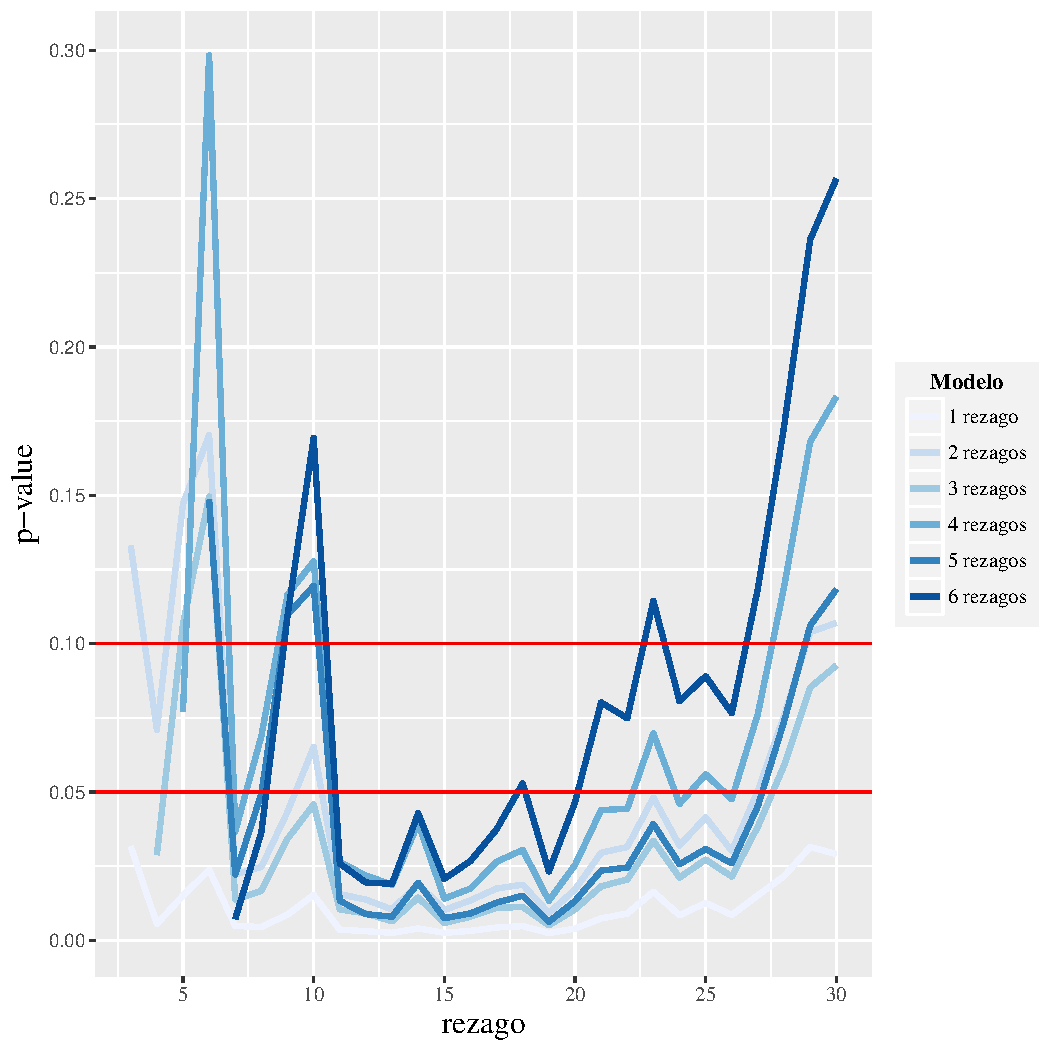
\includegraphics[width=5in,height=3.5in]{figure/unnamed-chunk-12-1} 

}

\caption[Número de Rezagos para el contraste de Independencia]{Número de Rezagos para el contraste de Independencia}\label{fig:unnamed-chunk-12}
\end{figure}


\end{knitrout}

\begin{knitrout}
\definecolor{shadecolor}{rgb}{0.969, 0.969, 0.969}\color{fgcolor}\begin{kframe}
\begin{verbatim}
## #############
## ###Model VECM 
## #############
## Full sample size: 459 	End sample size: 451
## Number of variables: 2 	Number of estimated slope parameters 30
## AIC -4809.357 	BIC -4681.901 	SSR 5.482757
## Cointegrating vector (estimated by ML):
##    mayorista supermercado    const
## r1         1    -1.082801 1.183784
## 
## 
##                       ECT                mayorista -1      
## Equation mayorista    -0.1505(0.0327)*** 0.0810(0.0525)    
## Equation supermercado 0.0196(0.0152)     0.0468(0.0244).   
##                       supermercado -1     mayorista -2     
## Equation mayorista    0.2356(0.1066)*     0.1087(0.0525)*  
## Equation supermercado -0.0593(0.0495)     0.0725(0.0244)** 
##                       supermercado -2     mayorista -3      
## Equation mayorista    0.1879(0.1061).     0.0484(0.0516)    
## Equation supermercado -0.0077(0.0493)     0.0517(0.0240)*   
##                       supermercado -3    mayorista -4       
## Equation mayorista    0.1159(0.1065)     -0.0137(0.0509)    
## Equation supermercado 0.0361(0.0494)     0.0092(0.0236)     
##                       supermercado -4    mayorista -5       
## Equation mayorista    0.0355(0.1048)     -0.1019(0.0506)*   
## Equation supermercado 0.0783(0.0486)     -0.0328(0.0235)    
##                       supermercado -5     mayorista -6     
## Equation mayorista    0.0550(0.1037)      0.0886(0.0507).  
## Equation supermercado -0.0158(0.0481)     0.0524(0.0235)*  
##                       supermercado -6    mayorista -7      
## Equation mayorista    0.1109(0.1018)     0.0487(0.0505)    
## Equation supermercado 0.0232(0.0473)     0.0525(0.0234)*   
##                       supermercado -7    
## Equation mayorista    0.0783(0.1009)     
## Equation supermercado -0.0236(0.0468)
\end{verbatim}
\end{kframe}
\end{knitrout}


\begin{table}[H]
\begin{center}
\begin{tabular}{@{}lrllll@{}}
\toprule
\multicolumn{1}{l}{} & \multicolumn{2}{c}{Estadístico} &
\multicolumn{3}{c}{Valores críticos} \\
\cmidrule(l){2-3} \cmidrule(l){4-6} \\
\multicolumn{1}{l}{$\mathcal{H}_0$} & \multicolumn{2}{c}{$p = 2$} &
\multicolumn{1}{l}{90\%}&
\multicolumn{1}{l}{95\%}&
\multicolumn{1}{l}{99\%}
\\
\midrule
$r \leq 1$  & \multicolumn{2}{c}{  2.66}  & 6.50 & 8.18 & 11.65\\
$r = 0$     & \multicolumn{2}{c}{ 49.54}  & 15.66 & 17.95 & 23.52\\
\bottomrule
\end{tabular}
\end{center}
\caption{Contraste de la \textit{la traza} de cointegración de Johansen}
\label{tab-10}
\end{table}


\begin{table}[H]
\begin{center}
\begin{tabular}{@{}lrllll@{}}
\toprule
\multicolumn{1}{l}{} & \multicolumn{2}{c}{Estadístico} & \multicolumn{3}{c}{Valores críticos} \\
\cmidrule(l){2-3} \cmidrule(l){4-6} \\
\multicolumn{1}{l}{$\mathcal{H}_0$} & \multicolumn{2}{c}{$p = 2$} &
\multicolumn{1}{l}{90\%}&
\multicolumn{1}{l}{95\%}&
\multicolumn{1}{l}{99\%}
\\
\midrule
$r \leq 1$ & \multicolumn{2}{c}{ 2.66} & 6.50 & 8.18 & 11.65\\
$r = 0$ & \multicolumn{2}{c}{46.88} & 12.91 & 14.90 & 19.19 \\
\bottomrule
\end{tabular}
\end{center}
\caption{Contraste del \textit{máximo autovalor} de cointegración de Johansen}
\label{tab-11}
\end{table}




\chapter{Procesos de transmisión asimétricos}
\section{Modelo de vectores de corrección del error por umbrales (TVECM)}
\begin{defin}
Una serie de tiempo $K$-dimensional $\bf{y}_{t}$ se dice que sigue un modelo TVECM de $k$-regímenes de orden $p$ si satisface
\begin{equation}
\Delta y_{t}=c_{j}+\bold{\Pi}_{j}\bf{y}_{t-1}+\bold{\Gamma}_{1j}\Delta \bf{y}_{t-1}+...+\bold{\Gamma}_{(p-1),j}\Delta \bf{y}_{t-p+1}+u_{tj}, \quad \text{si}\quad \gamma_{j-1}\leq y_{t-d-1}\leq \gamma_{j}
\end{equation}
\end{defin}
\subsection{El contraste de Hansen \& Seo (2002)}
Cuando estimamos un modelo TVECM resulta vital discernir si este modelo no lineal tiene una performance superior a la que tendría un modelo lineal VECM. Hansen \& Seo (2002) propusieron un contraste  

\subsection{Contrastes de linealidad}
\subsection{Estimación del modelo}
\subsection{Relaciones dinámicas a corto plazo}
\section{Resultados de la aplicación}
\subsection{Análisis de las relaciones asimétricas}
\subsection{Especificación del sistema}
\subsection{Estimación del modelo TVECM}
\subsection{Funciones de impulso respuesta}
\subsection{Diagnósticos del modelo}

\begin{knitrout}
\definecolor{shadecolor}{rgb}{0.969, 0.969, 0.969}\color{fgcolor}\begin{kframe}
\begin{verbatim}
## 59 (2.4%) points of the grid lead to regimes with percentage of observations < trim and were not computed
\end{verbatim}
\end{kframe}\begin{figure}[H]

{\centering 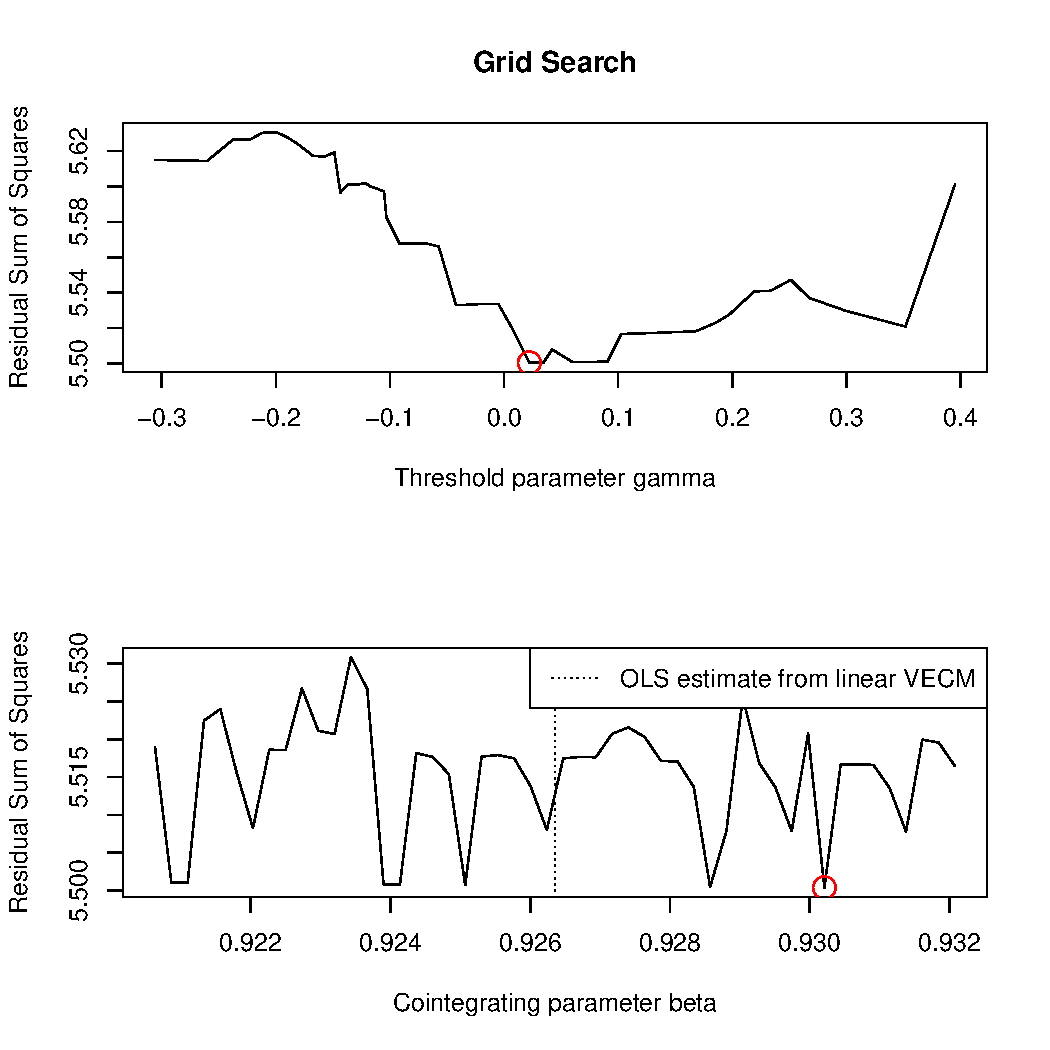
\includegraphics[width=4.5in,height=4.5in]{figure/fig-5-1} 

}

\caption[Modelo de corrección del error por umbrales]{Modelo de corrección del error por umbrales}\label{fig:fig-5}
\end{figure}


\end{knitrout}

%insert in the preamble and uncomment the line you want for usual /medium /small matrix
%\usepackage{amsmath} \newenvironment{smatrix}{\begin{pmatrix}}{\end{pmatrix}} %USUAL
%\usepackage{amsmath} \newenvironment{smatrix}{\left(\begin{smallmatrix}}{\end{smallmatrix}\right)} %SMALL
%\usepackage{nccmath} \newenvironment{smatrix}{\left(\begin{mmatrix}}{\end{mmatrix}\right)} %MEDIUM
\begin{equation}
\begin{smatrix} %explained vector
\Delta X_{t}^{1} \\ \Delta X_{t}^{2}
\end{smatrix}=
\left\{
\begin{array}{ll}
\begin{smatrix} %ECT
-0.0410 \\ 0.0565
\end{smatrix}ECT_{-1}+
\begin{smatrix}     %const
0.0060 \\ 0.0067
\end{smatrix}
+\begin{smatrix}      %Lag1
0.0705 & 0.2378 \\
0.0448 & -0.0519 
\end{smatrix}
\begin{smatrix}
\Delta X_{t-1}^{1} \\ \Delta X_{t-1}^{2}
\end{smatrix}
+\begin{smatrix}      %Lag2
0.0744 & 0.1690 \\
0.0563 & -0.0118 
\end{smatrix}
\begin{smatrix}
\Delta X_{t-2}^{1} \\ \Delta X_{t-2}^{2}
\end{smatrix}
+\begin{smatrix}      %Lag3
-0.0246 & 0.0674 \\
0.0394 & 0.0192 
\end{smatrix}
\begin{smatrix}
\Delta X_{t-3}^{1} \\ \Delta X_{t-3}^{2}
\end{smatrix}
& \text{if Th}< 0.233492973644388 \\
\begin{smatrix} %ECT
-0.1387 \\ -0.2280
\end{smatrix}ECT_{-1}+
\begin{smatrix}     %const
-0.0521 \\ 0.0748
\end{smatrix}
+\begin{smatrix}      %Lag1
0.0599 & 0.1583 \\
0.0611 & -0.0948 
\end{smatrix}
\begin{smatrix}
\Delta X_{t-1}^{1} \\ \Delta X_{t-1}^{2}
\end{smatrix}
+\begin{smatrix}      %Lag2
0.2173 & -0.0175 \\
0.1234 & -0.1118 
\end{smatrix}
\begin{smatrix}
\Delta X_{t-2}^{1} \\ \Delta X_{t-2}^{2}
\end{smatrix}
+\begin{smatrix}      %Lag3
0.3961 & 1.1882 \\
0.1269 & 0.1380 
\end{smatrix}
\begin{smatrix}
\Delta X_{t-3}^{1} \\ \Delta X_{t-3}^{2}
\end{smatrix}
& \text{if Th}> 0.233492973644388 \\
\end{array}
\right.
\end{equation}



\begin{knitrout}
\definecolor{shadecolor}{rgb}{0.969, 0.969, 0.969}\color{fgcolor}

{\centering 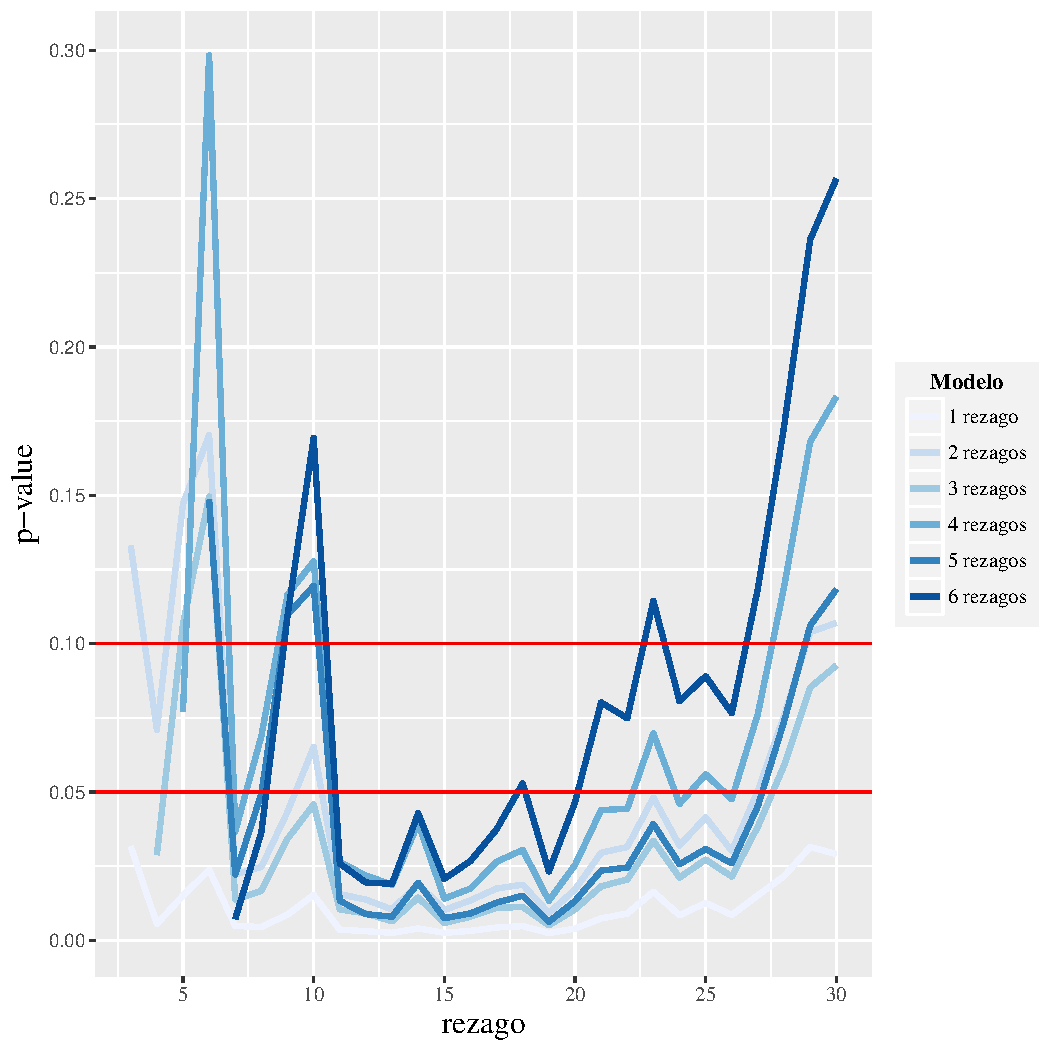
\includegraphics[width=4.5in,height=3.5in]{figure/unnamed-chunk-16-1} 

}



\end{knitrout}


\begin{knitrout}
\definecolor{shadecolor}{rgb}{0.969, 0.969, 0.969}\color{fgcolor}

{\centering 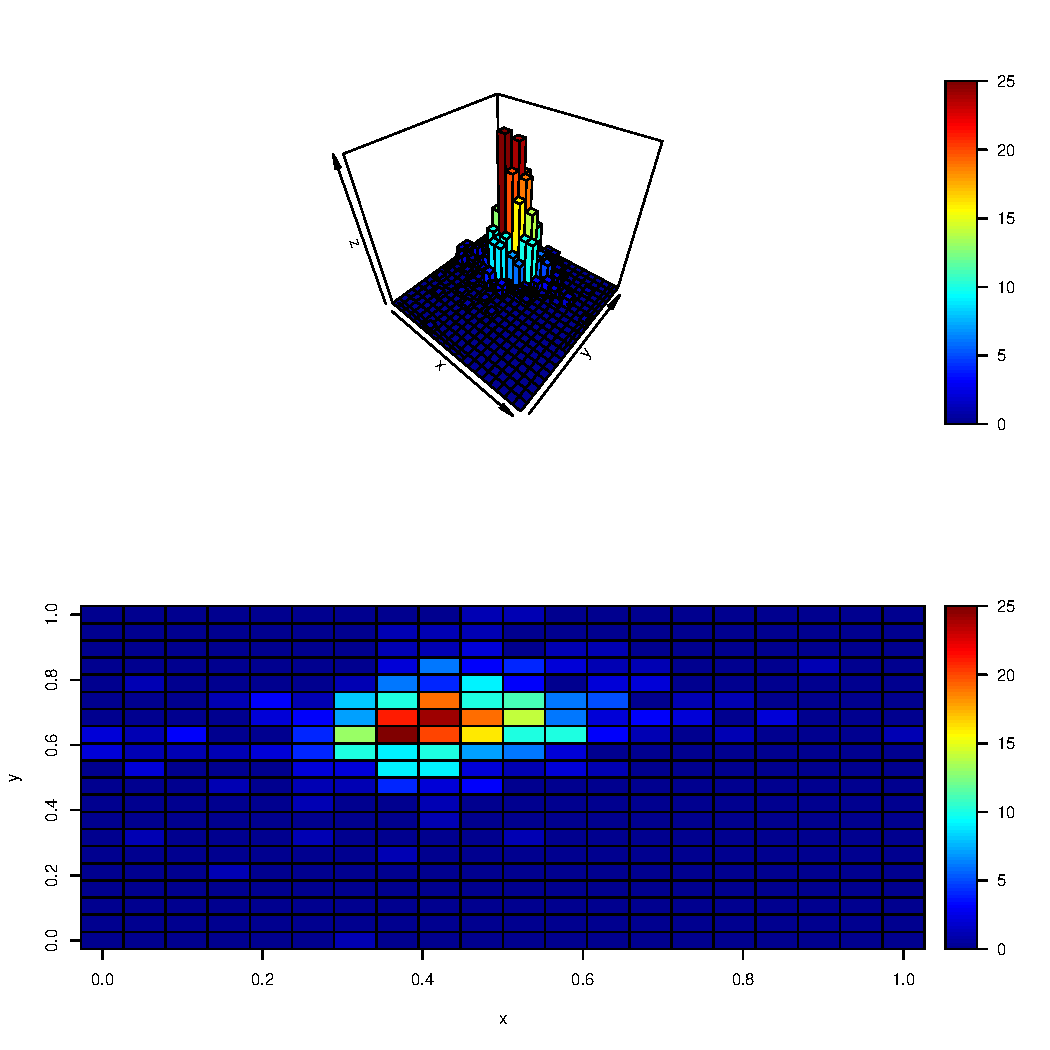
\includegraphics[width=4.5in,height=3.5in]{figure/unnamed-chunk-17-1} 

}



\end{knitrout}

\begin{knitrout}
\definecolor{shadecolor}{rgb}{0.969, 0.969, 0.969}\color{fgcolor}\begin{kframe}
\begin{verbatim}
## $JB
## 
## 	JB-Test (multivariate)
## 
## data:  Residuals of VAR object mono
## Chi-squared = 836.84, df = 4, p-value < 2.2e-16
## 
## 
## $Skewness
## 
## 	Skewness only (multivariate)
## 
## data:  Residuals of VAR object mono
## Chi-squared = 43.908, df = 2, p-value = 2.921e-10
## 
## 
## $Kurtosis
## 
## 	Kurtosis only (multivariate)
## 
## data:  Residuals of VAR object mono
## Chi-squared = 792.93, df = 2, p-value < 2.2e-16
## $multi
##         E df   P(Chi > E)
## 1 249.622  4 7.852179e-53
## 
## $univ
##                      E df   P(Chi > E)
## mayorista     72.66811  2 1.660813e-16
## supermercado 176.95389  2 3.757949e-39
\end{verbatim}
\end{kframe}
\end{knitrout}

\nocite{greene2003}

\chapter{Conclusiones}
\chapter{Bibliografía}

\printbibliography

\chapter{Anexo}
\begingroup
\renewcommand\thesection{A}
\titleformat{\section}[display]
{\normalfont\huge\bfseries}{}{20pt}{\huge}

\section{Desarrollos adicionales}
\subsection{Mínimos cuadrados multivariados}

Considere el siguiente modelo lineal multivariado 

\begin{equation}\label{MLS}
\bf{y}_{k} = \bf{C}\bf{x}_{k}+\boldsymbol{\varepsilon}_{k}, \quad k=1,...,T, 
\end{equation}

Donde $\bf{y}_{k}= (y_{1k},...,y_{mk})'$ es un vector de variables respuesta de dimensión $m\times 1$, $\bf{x}_{k}=(x_{1k},..,x_{nk})'$ es un vector de $n\times 1$ de predictores\footnote{pudiendo ser éstos tanto valores rezagados de $\bf{y}_{k}$ o variables exógenas}, $\bf{C}$ es una matriz de coeficienes de $m\times n$ y $\boldsymbol{\varepsilon}_{k}$ es un vector de $m\times 1$ errores aleatorios, con media $\mathbb{E}(\boldsymbol{\varepsilon}_{k})=\bf{0}$ y matriz de covarianzas $\text{Cov}(\boldsymbol{\varepsilon_{k}})=\bold{\Sigma}_{\varepsilon\varepsilon}$, una matriz de $m\times n$ definida positiva. Los elementos del vector $\boldsymbol{\varepsilon}_{k}$ son asumidos independientes para diferentes $k$. Asumiendo que se dispone de $T$ observaciones, podemos definir las siguientes matrices 
\begin{align}
\bf{Y} = \left[\bf{y}_{1},...,\bf{y}_{T} \right]_{m\times T} = \left[
\begin{array}{ccc} 
y_{11} & \hdots & y_{1T} \\ 
\vdots & \ddots & \vdots \\ 
y_{m1} & \hdots & y_{mT}
\end{array}\right] 
\end{align}

\begin{align}
\bf{X} = \left[\bf{x}_{1},...,\bf{x}_{T} \right]_{n\times T} = \left[
\begin{array}{ccc} 
x_{11} & \hdots & x_{1T} \\ 
\vdots & \ddots & \vdots \\ 
x_{m1} & \hdots & x_{mT}
\end{array}\right] 
\end{align}
Si se asume $m+n\leq T$ y que $\bf{X}$ es de rango completo $n=rank(\bf{X})<T$. Se apilan los vectores de errores para formar una matriz $m\times T$ 
$\boldsymbol{\varepsilon} = [\boldsymbol{\varepsilon}_{1},\boldsymbol{\varepsilon}_{2},...,\boldsymbol{\varepsilon}_{T}]$. De esta forma puede escribirse el modelo de manera compacta como

\begin{equation}
\underbrace{\bf{Y}}_{m\times T}=\underbrace{\bf{C}}_{m\times n}\underbrace{\bf{X}}_{n\times T}+\underbrace{\boldsymbol{\varepsilon}}_{m\times T}
\end{equation}
Otra forma de tratar la matriz de errores es a través del operador \textit{vec}, $T: \mathbb{R}^{m\times T}\rightarrow \mathbb{R}^{mT\times 1}$.
$e = (\boldsymbol{\varepsilon_{(1)}}, \boldsymbol{\varepsilon_{(2)}}, ..., \boldsymbol{\varepsilon_{(m)}})'$. Se formulan entonces los siguientes supuestos 

\begin{align}
\mathbb{E}(e) = \bf{0} && && \text{Cov}(e) = \bold{\Sigma}_{\varepsilon\varepsilon} \otimes \bf{I}_{T}
\end{align}


Donde $\otimes$ denota el producto de Kronecker\footnote{Sean $\bf{A}$ una matriz $n\times p$ y $\bf{B}$ una matriz $m\times q$. Entonces la matriz $mn\times pq$
\begin{equation}
\bf{A}\otimes \bf{B} = \left[
\begin{array}{cccc}
& & & \\
& & & \\ 
& & & 
\end{array}\right]
\end{equation}
}
\subsection{Regresión de Rango Reducido}
La regresión de rango reducido (RRR) es una técnica. Para el modelo descrito en  \eqref{MLS} se tiene que 

\begin{equation}
rank(\bf{C}) = r\leq min(n,m)
\end{equation}


\endgroup
\begingroup
\renewcommand\thesection{B}
\titleformat{\section}[display]
{\normalfont\huge\bfseries}{}{20pt}{\huge}
\section{Código R}
\subsection{Información de la sesión}
\begin{knitrout}\scriptsize
\definecolor{shadecolor}{rgb}{1, 1, 1}\color{fgcolor}\begin{kframe}
\begin{verbatim}
## R version 3.4.0 (2017-04-21)
## Platform: x86_64-pc-linux-gnu (64-bit)
## Running under: Ubuntu 16.04.2 LTS
## 
## Matrix products: default
## BLAS: /usr/lib/libblas/libblas.so.3.6.0
## LAPACK: /usr/lib/lapack/liblapack.so.3.6.0
## 
## locale:
##  [1] LC_CTYPE=es_CL.UTF-8       LC_NUMERIC=C              
##  [3] LC_TIME=es_CL.UTF-8        LC_COLLATE=es_CL.UTF-8    
##  [5] LC_MONETARY=es_CL.UTF-8    LC_MESSAGES=es_CL.UTF-8   
##  [7] LC_PAPER=es_CL.UTF-8       LC_NAME=C                 
##  [9] LC_ADDRESS=C               LC_TELEPHONE=C            
## [11] LC_MEASUREMENT=es_CL.UTF-8 LC_IDENTIFICATION=C       
## 
## attached base packages:
## [1] tcltk     stats     graphics  grDevices utils     datasets  methods  
## [8] base     
## 
## other attached packages:
##  [1] asbio_1.3-4        plot3D_1.1         RColorBrewer_1.1-2
##  [4] reshape2_1.4.2     ggplot2_2.2.1      tsDyn_0.9-44      
##  [7] vars_1.5-2         lmtest_0.9-35      strucchange_1.5-1 
## [10] sandwich_2.3-4     zoo_1.8-0          MASS_7.3-47       
## [13] uroot_2.0-9        urca_1.3-0         forecast_8.0      
## [16] bindrcpp_0.1       tidyr_0.6.3        dplyr_0.7.0       
## [19] magrittr_1.5       knitr_1.16.5      
## 
## loaded via a namespace (and not attached):
##  [1] deSolve_1.14         lattice_0.20-35      colorspace_1.3-2    
##  [4] mgcv_1.8-17          rlang_0.1.1          glue_1.0.0          
##  [7] TTR_0.23-1           foreach_1.4.3        bindr_0.1           
## [10] plyr_1.8.4           multcompView_0.1-7   quantmod_0.4-10     
## [13] stringr_1.2.0        timeDate_3012.100    munsell_0.4.3       
## [16] tseriesChaos_0.1-13  gtable_0.2.0         mvtnorm_1.0-6       
## [19] codetools_0.2-15     evaluate_0.10        misc3d_0.8-4        
## [22] tseries_0.10-41      parallel_3.4.0       highr_0.6           
## [25] xts_0.9-7            Rcpp_0.12.11         scales_0.4.1        
## [28] plotrix_3.6-5        scatterplot3d_0.3-40 fracdiff_1.4-2      
## [31] mnormt_1.5-5         digest_0.6.12        stringi_1.1.5       
## [34] grid_3.4.0           quadprog_1.5-5       tools_3.4.0         
## [37] lazyeval_0.2.0       tibble_1.3.3         pkgconfig_2.0.1     
## [40] Matrix_1.2-10        assertthat_0.2.0     iterators_1.0.8     
## [43] pixmap_0.4-11        R6_2.2.1             nnet_7.3-12         
## [46] nlme_3.1-131         compiler_3.4.0
\end{verbatim}
\end{kframe}
\end{knitrout}

\subsection{Importación y depurado de los datos}



\subsection{Selección modelo VAR}



\subsection{Función normalidad}



\endgroup

\end{document}
